% $Author: Luc $
% $Date: 2008-11-09 11:14:31 +0200 (Sun, 09 Nov 2008) $
% $Revision:  $
%=================================================================
\ifx\wholebook\relax\else
% --------------------------------------------
% Lulu:
    \documentclass[a4paper,10pt,twoside]{book}
    \usepackage[
        papersize={6in,9in},
        hmargin={.75in,.75in},
        vmargin={.75in,1in},
        ignoreheadfoot
    ]{geometry}
    \input{../common.tex}
    \pagestyle{headings}
    \setboolean{lulu}{true}
% --------------------------------------------
% A4:
%   \documentclass[a4paper,11pt,twoside]{book}
%   \input{../common.tex}
%   \usepackage{a4wide}
% --------------------------------------------
    \graphicspath{{figures/} {../figures/}}
    \begin{document}
%   \renewcommand{\nnbb}[2]{} % Disable editorial comments
    \sloppy
\fi

\chapter{Boucle}\label{cha:looping}

\noindent\hrule

\includegraphics[width=0.9\textwidth]{loopTitlePicture}
\noindent\hrule\vspace{1.5cm}

A présent, vous devez penser que le travail de programmeur de robot est assez 
fastidieux. Vous avez probablement un certain nombre d'idées pour des dessins 
intéressants, mais seulement, vous n'avez pas le courage d'écrire des scripts 
pour les dessiner, en effet, il semble que le nombre de lignes que vous avez à 
taper devient de plus en plus grand lorsque la complexité du dessin augmente. 
Dans ce chapitre, vous apprendrez à utiliser des boucles afin de réduire le nombre 
des expressions donné à un robot. Des boucles vous permettent de répéter une 
séquence d'expressions. Avec une boucle, le script pour le dessin d'un hexagone 
ou un octogone n'est pas plus long que le script du dessin d'un carré.

\section{Une Etoile est Née} 

Nous voudrions demander à un robot de dessiner une étoile, semblable à celle montrée 
dans l'image au début de ce chapitre. Nous allons charger pica de dessiner une étoile 
de la manière suivante: à partir de ce que sera le centre de l'étoile, tracer une 
ligne, retourner au centre, tourner d'un certain angle, tirer une autre ligne, et ainsi 
de suite jusqu'à ce que l'étoile soit finie. Le Script~\ref{scr:71} crée un robot qui 
trace une ligne d'une longueur de 70 pixels, puis retourne à son emplacement 
précédent. Notez qu'une fois qu'il est retourné à son point de départ, le robot effectue 
un volte-face, de sorte qu'il soit orienté dans sa direction initiale.

\begin{script}[71]{Dessiner une ligne et repartir }
| pica | 
pica := Bot new. 
pica go: 70. 
pica turnLeft: 180. 
pica go: 70. 
pica turnLeft: 180.
\end{script}

Pour dessiner une étoile, nous avons repris une partie du Script~\ref{scr:71} et ensuite 
demandé au robot de tourner pour un angle donné. Dessinons une étoile à six pointes, ainsi 
l'angle sera de 60 degrés, en effet tourner de 60 degrés à chaque fois se traduira par 
360 / 60 = 6 branches. Le Script~\ref{scr:72} montre comment faire pour obtenir une étoile 
à 6 branches, sans l'aide de boucles. 


\begin{script}[72]{Une étoile à 6 branches sans boucles}
| pica | 
pica := Bot new. 
pica go: 70. 
pica turnLeft: 180. 
pica go: 70. 
pica turnLeft: 180. 
pica turnLeft: 60. 
pica go: 70. 
pica turnLeft: 180. 
pica go: 70. 
pica turnLeft: 180. 
pica turnLeft: 60. 
pica go: 70. 
pica turnLeft: 180. 
pica go: 70. 
pica turnLeft: 180. 
pica turnLeft: 60. 
pica go: 70. 
pica turnLeft: 180. 
pica go: 70. 
pica turnLeft: 180. 
pica turnLeft: 60. 
pica go: 70. 
pica turnLeft: 180. 
pica go: 70. 
pica turnLeft: 180. 
pica turnLeft: 60. 
pica go: 70. 
pica turnLeft: 180. 
pica go: 70. 
pica turnLeft: 180. 
pica turnLeft: 60.
\end{script}

Comme vous pouvez le voir, après que pica soit créé, il répète les mêmes cinq lignes de 
code à six reprises (affiché en alternance de type romain et en italique). Cela parait 
superflu d'avoir à taper le même segment de code je ne sais combien de fois. Imaginez la 
longueur de votre script si vous vouliez une étoile à 60 branches, comme celui montré dans 
l'exercice ~\ref{xp:71}. Nous avons donc besoin d'une technique pour répéter une séquence d'expressions.

\section{Des Boucles à la Rescousse} 

La solution à notre problème est d'utiliser une boucle. Il existe différents types de 
boucles, et celui que je vais présenter ici vous permet de répéter une séquence de messages 
donnés un certain nombre de fois. La méthode \ct{timesRepeat:} répète une séquence d'expressions 
un nombre de fois donné, comme indiqué dans le Script~\ref{scr:73}.Ce script définit la même étoile que celle du Script~\ref{scr:72}, 
mais avec beaucoup moins de code. Notez que les expressions répétées sont entre crochets.

Script~\ref{scr:73}.

\begin{script}[73]{Dessin d'une étoile à 6 branches en utilisant une boucle}
| pica | 
pica := Bot new. 
6 timesRepeat: 
	!\textbf{[ pica go: 70.}!
	!\textbf{pica turnLeft: 180. }!
	!\textbf{pica go: 70. }!
	!\textbf{pica turnLeft: 180. }!
	!\textbf{pica turnLeft: 60 ] }!
\end{script}


\important{\ct{n timesRepeat: [ s\'equence d'expressions ]} répète une séquence d'expression n fois.}

La méthode \ct{timesRepeat:} vous permet de répéter une séquence d'expressions, et dans Smalltalk, 
comme une séquence d'expressions, délimité par des crochets, est appelée  \emph{bloc}. 

Le message \ct{timesRepeat:}est envoyé à un nombre entier, le nombre de fois que la séquence doit 
être répétée. Dans le Script~\ref{scr:73} le message \ct{timesRepeat: [...]} est envoyé à 
l'entier 6. Il n'y a rien de nouveau ici, vous avez un message envoyé à un nombre entier 
et nous avons examiné que : le second entier a été envoyé au premier, qui a retourné la somme. 

Enfin, notez que le nombre qui reçoit le message \ct{timesRepeat:}doit être un\emph{nombre entier}, 
parce que dans une boucle comme dans la vie réelle, cela n'aurait aucun sens 
de vouloir exécuter une séquence d'expressions 0,2785 fois. 

L'argument de \ct{timesRepeat:} est un bloc, qui est, une suite d'expressions entre crochets. 
Rappel du chapitre 2 que l'argument d'un message contient des renseignements nécessaires à 
l'objet de réception pour l'exécution du message. Par exemple, \ct{[ pica go: 70. pica turnLeft: 180. pica go: 70. ]} 
est un bloc composé de trois expressions \ct{pica go: 70, pica turnLeft: 180, and pica go: 70}. 

\important{L'argument de \ct{timesRepeat:} est un block, qui est, une séquence d'expressions 
entre crochets.} 


\section{Boucles au Travail} 

Si vous comparez le Script~\ref{scr:71} avec les expressions dans la boucle du  Script~\ref{scr:73}, 
vous verrez qu'il ya une expression supplémentaire: \ct{pica turnLeft: 60}, qui crée l'angle 
entre les branches adjacentes. Il existe une relation simple entre le nombre de branches et 
l'angle par lequel le robot doit tourner avant de dessiner la branche suivante : Pour une 
étoile complète, la relation entre l'angle et le nombre de répétitions doit être 
$angle*n = 360$. 

Pour adapter le Script~\ref{scr:73} afin de dessiner une étoile avec un autre nombre de branches, 
il faut changer le nombre de fois que la boucle est répétée en remplaçant $6$ par l'entier approprié. 
Notez que l'angle de $60$ devrait également être modifié si vous souhaitez générer une étoile complète. 

\begin{exofigwithsizeandtitle}[0.65]{
\includegraphics[width=3.5cm]{loopStar60}}{Une Etoile à Soixante Branches}\label{xp:71}
Ecrivez un script qui dessine une étoile à 60 branches. 
\end{exofigwithsizeandtitle}

\section{L’indentation du Code} 

Le code Smalltalk peut être disposé de manières variées, et son indentation de la marge 
gauche n'a pas d'effet sur la façon dont le code est exécuté. Nous disons que l'indentation 
n'a aucun effet sur la syntaxe ``au sens''  du programme. Cependant, l’utilisation de 
l'indentation claire et cohérente aide le lecteur à comprendre le code. 


Je vous suggère de suivre la convention qui a été utilisé dans le Script~\ref{scr:73} pour la mise 
en forme de l’expression \ct{timesRepeat:} :. L'idée est que le bloc répété conprenant les expressions 
délimitées par les caractères[ and ] doit former un rectangle visuelles et textuelles. C'est 
pourquoi le bloc commence par le crochet de gauche sur la ligne suivant \ct{timesRepeat:}et 
ensuite nous alignons toutes les expressions à l'intérieur du bloc de la largeur d’une 
tabulation. Le crochet droit à la fin indique que le bloc est terminé. La Figure 
~\ref{fig:71} devrait vous convaincre que le code indenté est plus facile à lire que le code 
non indenté.

\begin{figure}[htbp]
	\centering
		\includegraphics[width=.9\linewidth]{indent}
	\caption{Une indentation des blocks rend plus facile l’identification des boucles. A gauche : 
	non indenté. A droite : indenté.}
	\label{fig:71}
\end{figure}


Le code de mise en forme est un sujet de discussion sans fin, parce que les gens aiment 
lire leur code de différentes manières. La convention que je propose se concentre 
principalement sur  l'aide à l'identification des expressions répétées.
 
\section{Dessin de Figures Géométriques Régulières} 

Beaucoup de figures peuvent être obtenues par de simples séquences de messages répétées, 
telles que le carré qui a été dessiné dans le chapitre ~\ref{cha:turning} (repris ici par le Script~\ref{scr:74}). 

\begin{script}[74]{Le Premier Carré de Pica}
| pica | 
pica := Bot new. 
pica go: 100. 
pica turnLeft: 90. 
pica go: 100. 
pica turnLeft: 90. 
pica go: 100. 
pica turnLeft: 90. 
pica go: 100. 
pica turnLeft: 90
\end{script}


\begin{exonofigtitle}{Un Carré utilisant une Boucle}
Transformez le Script~\ref{scr:72} afin qu’il dessine le même carré tout en utilisant la 
commande \ct{timesRepeat:}. Maintenant, vous devriez être capable de dessiner d'autres 
polygones réguliers, même ceux avec un grand nombre de côtés.
\end{exonofigtitle}


\begin{exofigwithsizeandtitle}[0.65]{\includegraphics[width=3.5cm]{loopPentagon}}{Un Pentagone Régulier}\label{xp:73}
Dessinez un pentagone régulier en utilisant la méthode \ct{timesRepeat:}. 
\end{exofigwithsizeandtitle}


\begin{exofigwithsizeandtitle}[0.65]{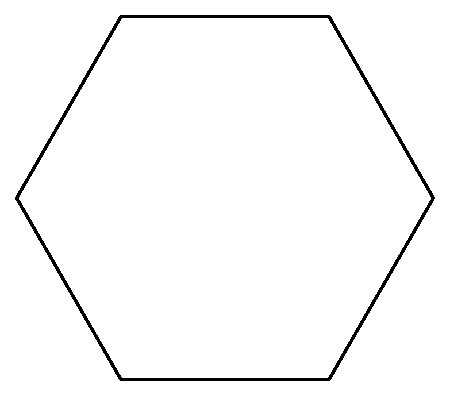
\includegraphics[width=3.5cm]{loopHexagon}}{Un Hexagone Régulier}\label{xp:74}
Dessinez un hexagone régulier en utilisant la méthode \ct{timesRepeat:}.
\end{exofigwithsizeandtitle}

Une fois que vous avez obtenu ces polygones, essayez de dessiner un polygone régulier avec 
un très grand nombre de côtés. Vous pourriez avoir à réduire la longueur des côtés dans le 
but de faire passer la figure dans l'écran. Lorsque le nombre de côtés est grand et la 
longueur du côté est de petite taille, le polygone ressemble à un cercle.


\section{Redécouvrir les Pyramides} 

Rappelez vous comment vous avez codé le contour de la pyramide de Saqqarah dans l'exercice
~\ref{xp:saqq}. Vous pouvez simplifier votre code en utilisant une boucle, comme indiqué 
dans le Script~\ref{scr:75}. 


\begin{scriptfigwithsize}[0.4]{\includegraphics[width=5cm]{loopPyramid}}{Un script de pyramide utilisant des boucles}\label{scr:75}
| pica | 
pica := Bot new. 
5 timesRepeat: 
	[pica north. 
	pica go: 20. 
	pica east. 
	pica go: 20]. 
5 timesRepeat: 
	[pica go: 20. 
	pica south. 
	pica go: 20. 
	pica east]. 
pica west. 
pica go: 200. 
\end{scriptfigwithsize}

Maintenant, vous devriez être en mesure de générer des pyramides avec un nombre arbitraire 
de terrasses en utilisant le même nombre d'expressions, simplement en changeant les 
chiffres dans le script. 


\begin{exofigwithsizeandtitle}[0.55]{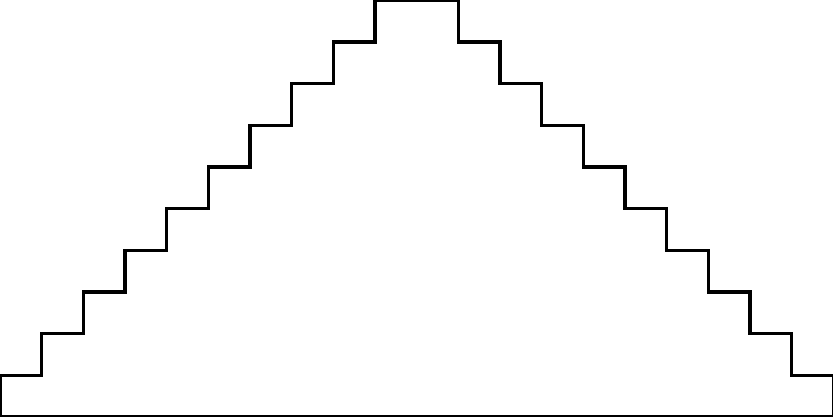
\includegraphics[width=4.5cm]{loopPyramid10}}{Une Pyramide à Dix Marches}
Dessiner une pyramides avec 10 terrasses en utilisant une variant du Script~\ref{scr:75}. 
\end{exofigwithsizeandtitle}

Vous pouvez maintenant générer des pyramides avec un plus grand nombre de terrasses. La taille des terrasses 
devra être ajusté, si vous voulez qu’elle soit de la même taille que l'écran. 


\section{Encore plus d’Exercices avec des Boucles } 

Comme vous l'avez vu, générer une pyramide à degrés implique la répétition d'un bloc de 
code qui dessine deux segment. Une fois que vous avez identifié le bon élément répété, 
vous pouvez produire des images complexes à partir de dessins élémentaires répétés. Les 
exercices suivants illustrent ce principe. 

\begin{exofigwithsizeandtitle}[0.65]{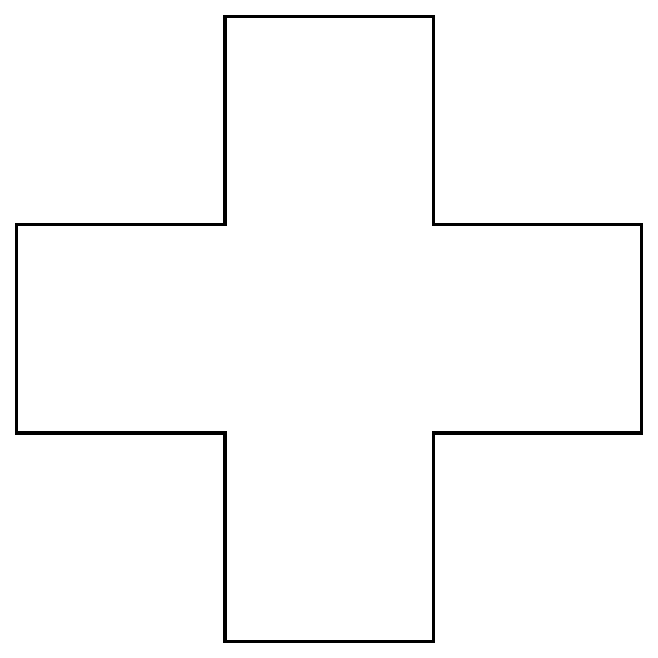
\includegraphics[width=3.5cm]{loopCross}}{Une Croix Suisse}
Dessinez le contour de la croix suisse figurant à droite en utlisant \ct{turnLeft:} oo \ct{turnRight:} et \ct{timesRepeat:}.
\end{exofigwithsizeandtitle}

\begin{exofigwithsizeandtitle}[0.65]{
\includegraphics[width=3.5cm]{loopStair}}{Un Escalier}
Dessinez l’escalier représenté sur la figure. 
\end{exofigwithsizeandtitle}

\begin{exofigwithsizeandtitle}[0.65]{
\includegraphics[width=3.5cm]{loopStylisedStair}}{Un Escalier sans Contremarches} 
Dessinez  l’escalier stylé—avec marches mais sans contremarches—illustré sur  la figure.
\end{exofigwithsizeandtitle}

\begin{exofigwithsizeandtitle}[0.65]{
\includegraphics[width=.5cm]{loopSimpleElement}}{Une Agrafe} 
Dessinez  l’élément graphique illustré qui ressemble à une agrafe.
\end{exofigwithsizeandtitle}

\begin{exofigwithsizeandtitle}[0.55]{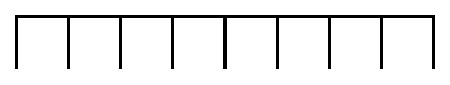
\includegraphics[width=4cm]{loopComb}}{Un Peigne} 
Transformez l’élément graphique que vous avez réalisé dans l’Exercice 7-9 afin de créer un peigne comme le montre la figure.
\end{exofigwithsizeandtitle}

\begin{exofigwithsizeandtitle}[0.65]{
\includegraphics[width=0.7cm]{loopLadder}}{Une Echelle}
Transformez l’élément graphique de  l’Exercice 7-9 afin de créer une échelle. 
\end{exofigwithsizeandtitle}

\begin{exonofigtitle}{Un Carré Dégringolant} 
Maintenant que vous maîtrisez les boucles en utilisant timesRepeat:, définissez  une boucle qui dessine 
les carrés dégringolant illustré au début du chapitre 4. 
\end{exonofigtitle}


\section{Résumé} 

Dans ce chapitre vous avez appris comment programmer des boucles en utilisant la méthode \emph{n} \ct{timesRepeat:}. 

\vspace*{5mm}
\noindent
\setlength{\extrarowheight}{1mm}
{\small \begin{tabular}{p{14mm}p{23mm}p{45mm}p{22mm}}
\hline
\textbf{Méthode} & \textbf{Syntaxe} & \textbf{Description} & \textbf{Exemple}\\
\hline
\textsf{timesRepeat:} & \textsf{n timesRepeat: [une séquence d'expressions]} & répère une séquence d'expression n fois & 
\textsf{10 timesRepeat: [ pica go: 10. 
pica jump: 10 ]}\\
\hline
\end{tabular}}









\ifx\wholebook\relax\else\end{document}\fi